
The EUDET-type beam telescopes are tabletop tracking detectors featuring six pixelated silicon sensors, four scintillators with photo multiplier tubes (PMTs) for trigger purposes,
 a Trigger Logic Unit (TLU) providing trigger logic and time stamp information on particle passage, and a data acquisition system for the readout. 
Figure\,\ref{fig:datura-tscope} shows the beam telescope with its rectangular aluminium sensor jigs, wherein the pixel sensors are embedded,
 and its auxiliary boards providing connections for power, sensor configuration, clock signals and data transmission. 
The planes are organised in two telescope arms holding three sensors each. 
A DUT can be inserted between the arms or at either end of the beam telescope. 
In the Cartesian, right-handed coordinate system chosen, the $y$-direction points vertically down and the $z$-direction along the beam direction.

\begin{figure}[tb]
	\center
	\ifdefined\notFOREPJ
	\includegraphics[width=.9\textwidth]{figures/DATURA2a.jpg}
	\else
	\includegraphics[width=.9\textwidth]{DATURA2a.jpg}
	\fi
	\caption[The $\Datura$ telescope]{The $\Datura$ beam telescope with its sensor planes (green frame) on aluminium rails.
	The auxiliary boards (red frame) with connections for clock, sensor configuration, and data are mounted at the top of the planes.
	Coolant is provided to the planes via tubes.}
	\label{fig:datura-tscope}
\end{figure}
 
\subsection{Sensors and mechanics}
\label{sec:sensors}

The $\Mimosa$ sensors used for precise spatial measurements of particle trajectories are manufactured with the AMS 350\,nm CMOS technology~\cite{HuGuo2010480}. 
Each $\Mimosa$ sensor consists of pixels sized $\unit{18.4}{\upmu\meter}\,\times\,\unit{18.4}{\upmu\meter}$, which are arranged in 1152 columns and 576 rows.
This adds up to a total of about six hundred thousand readout channels per sensor, covering an active area of about $\unit{10.6}{\milli\meter}\,\times\,\unit{21.1}{\milli\meter}$. 
The specifications of the $\Mimosa$ sensors quote a thickness of $\unit{50}{\upmu\meter}$. 
Measurements with a digital microscope reveal an average thickness over the six sensors used of $(54.5\,\pm\,3.6)\,\upmu\meter$. 
Free charge carriers produced in the underlying \unit{20}{\upmu\meter} high resistivity (about 400\,$\Omega$cm) epitaxial layer\footnote{This is the case for DATURA.} %Other beam telescopes are equipped with sensors differing slightly in epitaxial thickness.
 are collected via drift (diffusion) in depleted (undepleted) regions. 
The binary resolution of $\unit{5.3}{\upmu\meter}$ is improved by charge sharing, i.e.\ the collection of charge at adjacent pixels and subsequent calculation of the centre of gravity,
 as is shown in section~\ref{sec:trackres}.
%With the rising industrial interest in high resistivity epitaxial silicon for CMOS detectors the production cost of improved noise and radiation hardness parameters
% became already possible with ~400 Ohm·cm for 10 μm epitaxial layer for $\Mimosa$. 

The $\Mimosa$ sensors are read out with a rolling-shutter, taking 16\,cycles of an 80\,MHz clock per row, with all columns being read out in parallel. 
This allows for correlated double sampling and zero suppression on-chip with the digital circuitry placed outside the active pixel array. 
At this clock frequency, the $\Mimosa$ integration time equals $\unit{115.2}{\upmu\second}$, allowing for about 8680 frames to be read out per second. 
The expected maximum rate of detectable particles through the active area is estimated to be about $\unit{1}{\mega\hertz/\centi\meter^2}$ due to the limited on-chip buffer size. 
The detection threshold is programmable via so-called JTAG files. 
These provide configurations with different threshold levels in integer multiples $\noise$ of the RMS noise of the individual planes. 
A sensor threshold setting of $\noise = 6$ therefore corresponds to a collected charge in a single pixel of at least six times the noise. 
At this threshold, the average noise occupancy per pixel is measured to be about $6\cdot10^{-5}$ per readout frame at room temperature~\cite{ref:mimosa26}.

Every pixel sensor is mounted within an aluminium jig, three jigs are in turn mounted on each of the two aluminium arms. 
The jigs feature a beam window around the position of the sensor location, minimising the material budget. 
Lightproof Kapton foils of $\unit{25}{\upmu\meter}$ thickness protect the sensors on each side.
The overall material of the beam telescope thus amounts to $\unit{300}{\upmu\meter}$ of silicon and $\unit{300}{\upmu\meter}$ of Kapton. 
The two telescope arms, usually one up- and one downstream of the DUT, are movable along the direction of the beam in order to allow for variably sized DUTs to be fitted into the set-up. 
The minimal distance between two sensors is given by the jig thickness of 20\,mm, the maximal distance is restricted by the length of the aluminium arms to 150\,mm at equidistant spacing.
Furthermore, the jigs are cooled keeping the $\Mimosa$ sensors at a constant temperature of typically 18$\,\celsius$ for stable operation.
The entire beam telescope is placed on a rotatable frame easing adjustment of its orientation parallel to the beam. 
Additionally, this frame is mounted on a sturdy structure providing stability over time and wheels for easy transportation. 

\begin{figure}[tb]
	\center
	\ifdefined\notFOREPJ
	\includegraphics[width=.9\textwidth]{figures/sketch_tscope6.eps}
	\else
	\includegraphics[width=.9\textwidth]{sketch_tscope6.eps}
	\fi
	\caption[Sketch of the $\DESY$-type telescope set-up]{Sketch of the $\DESY$-type telescope set-up and its important parameters.
	Planes 0 to 2 and planes 3 to 5 are referred to as upstream and downstream planes, respectively.}
	\label{fig:datura_sketch}
\end{figure}

Important parameters are compiled in figure~\ref{fig:datura_sketch}. 
The distance between $\Mimosa$ planes is denoted as $\dz$, the distance between the DUT and its nearest neighbouring $\Mimosa$ planes $\dzdut$. 
The $z$-positions of the pixel planes are denoted $z_0$ to $z_5$ and the DUT is placed at $z_{\textrm{DUT}}$. 
The expression $\varepsilon = \sum_i x_{i}/X_{0,i}$ defines the material budget of the scattering medium as the physical material thicknesses $x_i$ normalised to their radiation lengths,
 with values of $X_0 = 93.65\,\milli\meter$ for silicon, $X_0 = 3.042\cdot 10^{5}\,\milli\meter$ for dry air, and $X_0 = 285.6\,\milli\meter$ for Kapton, cf.~table~III.6 of reference \cite{ref:x0values}.
The material budget of a $\Mimosa$ plane including a protecting Kapton foil on each side is $\epsmimo = 7.5\cdot10^{-4}$ at an assumed sensor thickness of $\unit{54}{\upmu\meter}$. 
At a spacing of $\dz = \unit{20}{\milli\meter}$ ($\dz = \unit{150}{\milli\meter}$) the total material budget amounts to $4.8\cdot10^{-3}$ ($7.0\cdot10^{-3}$).
Likewise, $\epsdut$ represents the DUT's material budget which includes the DUT itself and other material such as PCBs and cooling boxes.

\subsection{Trigger and DAQ system}
\label{sec:tdaq}

Four Hamamatsu PMT assemblies with scintillators and lightguides, two in front and two in the back of the telescope, define the spatial acceptance for triggers. 
The crossed scintillators on either side of the beam telescope define a rectangular acceptance window of $10\,\milli\meter\,\times\,20\,\milli\meter$ matching the $\Mimosa$ sensor area. 
The TLU is based on a commercial Spartan\,3 board and features a coincidence unit with discriminator boards accepting up to four PMT input signals. 
Additionally, it is equipped with several custom-made add-on PCBs allowing for an easy integration of user DAQ systems. 
Providing a programmable logic, the TLU  takes a trigger decision based on its four input channels. 
As interface to the beam telescope DAQ and other user DAQs, the TLU provides RJ45 connectors with four LVDS pairs carrying the trigger clock, busy, reset, and trigger signals. 
The trigger clock and the busy line are inputs to the TLU, whereas the reset and the trigger line are signals produced by the TLU. 
The trigger signal is distributed to all DAQ systems on the trigger line. 
A busy signal is accepted by the TLU from each integrated DAQ individually vetoing subsequent triggers as long as the busy signal is high. 
More details are available in references~\cite{EUDET-2009-04,ref:TLUproc}.
%The reset line transmits the signal to reset the timestamp counter.
%The rising edges of the trigger clock are used as clock enable for the shift register holding the trigger data. 
In addition, a LEMO interface is available providing trigger and reset outputs and inputs for the busy signal.

Three different handshake modes handling the trigger/busy signals are available, one of them being the \textit{no-handshake mode},
 in which the TLU issues a fixed-length pulse on the trigger line with the busy line being disregarded. 
In \textit{simple handshake mode}, the assertion of a trigger is replied by the integrated DAQ systems by asserting a signal on the busy line. 
The TLU then de-asserts the trigger and waits for the busy line going low.
The \textit{trigger data handshake mode} uses the same scheme as in the \textit{simple handshake mode}, but additionally the current trigger data are transferred on the trigger line:
after the trigger has been de-asserted, the trigger number is clocked out. 
%
%The $\Mimosa$ sensors provide zero-suppressed hit data over a ribbon cable to the auxiliary boards,
% which provide RJ45 connectors to connect with the data concentrator board collecting the data from all six sensors and the trigger/busy lines from the TLU. 
%A 52-pin cable then transports the data and the TLU trigger/busy lines in parallel for the six $\Mimosa$ sensors into a FlexRIO board, which is equipped with a LVDS digital interface module
%  and an FPGA handling the $\Mimosa$ serial protocol. 
%The $\Mimosa$ data from the rolling-shutter readout is written continuously to RAM without taking into account the trigger information. 
%The data are then available via direct memory access to the DAQ software framework and an event is written to disk in normal handshake mode, only if a trigger has been raised for a certain telescope readout frame. 

The zero-suppressed hit data generated by the $\Mimosa$ sensors are transmitted over a ribbon cable to the auxiliary boards,
 which establish the connection to the data concentrator board collecting the data from all six sensors and the trigger/busy lines from the TLU.
The signals from the concentrator board are acquired by a COTS\footnote{commercial off-the-shelf} DAQ system built around the National Instrument (NI) PXIe crate architecture. 
A custom-made firmware running on a Virtex~5 FPGA embedded in a FlexRIO board (PXIe 7962R) acquires and deserialises the 12 serial links -- two per sensor -- at 80\,Mb/s,
 detects triggers on the trigger line and reads the trigger data, which are the bottom 15 bits of the trigger counter. 
The resulting data stream of 960 Mb/s is read by the CPU (PXIe 8130) from the PXIe bus via a DMA channel and processed on-line by software. 
Data packets on which the TLU has triggered are selected, demultiplexed and actual frames built. 
The data are then available to the $\eudaq$ framework (cf.\ section~\ref{sec:eudaq}), and an event is written to disk in normal handshake mode, only if a trigger has been raised for a certain telescope readout frame. 
This co-development, i.e.\ sharing processing tasks between firmware and software, allows for high flexibility for system upgrades. 
The presented DAQ architecture is able to read six $\Mimosa$ sensors without any dead-time at up to 8680 frames/s.
More details are available in references~\cite{EUDET-2010-25,Claus}.
 
 
